\documentclass[11pt]{scrartcl}
\usepackage{ngerman}	%Benutzung deutscher Umlaute
\usepackage{pgf}		%Zum Einbinden von JPEG
\usepackage{amsmath}	%Einrücken von Gleichungen z.B. durch gather
\usepackage{framed}

\author{Alex Jäger}
\title{Formelsammlung Hochfrequenztechnik}
\date{\today}
 

\begin{document}

\maketitle
\newpage
\section{Leitungstheorie}
\subsection{Leitungsmodell}
\begin{center}
	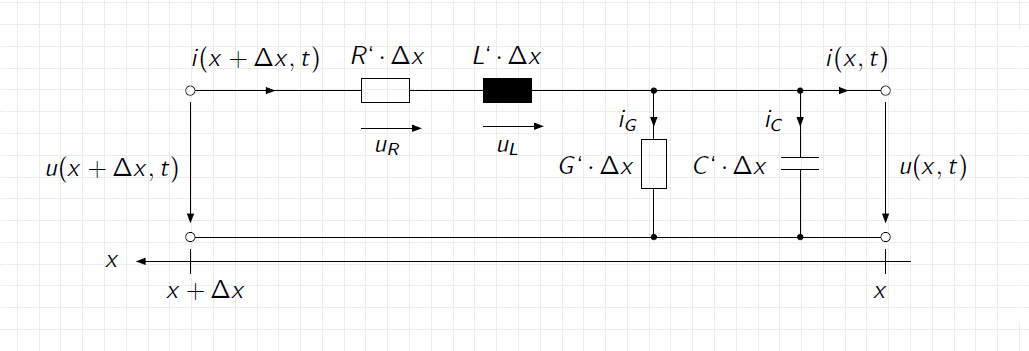
\includegraphics[width=\textwidth]{Grafiken/01_Leitungsmodell.png}
\end{center}
Kirchhoff'sche Regel führt z.B. zu
\begin{gather*}
	u_R+u_L+u(x,t)-u(x+\Delta x,t)=0 \\	
	R'*\Delta x*i(x+\Delta x,t)+L'*\Delta x*\frac{\partial i(x+\Delta x,t)}{\partial t}+u(x,t)-u(x+\Delta x,t)=0
\end{gather*}
oder
\begin{gather*}
	i(x+\Delta x,t)-i_g-i_c-i(x,t)=0 \\
	i(x+\Delta x,t)-G'*\Delta x*u(x,t)-C'*\Delta x*\frac{\partial u(x,t)}{\partial t}-i(x,t)=0
\end{gather*}
\begin{framed}
	\subsection{Telegraphengleichungen}
	\begin{eqnarray}
		\frac{\partial u(x,t)}{\partial x}=R'*i(x,t)+L'*\frac{\partial i(x,t)}{\partial t}\\
		\frac{\partial i(x,t)}{\partial x}=G'*u(x,t)+C'*\frac{\partial u(x,t)}{\partial t}
	\end{eqnarray}
\end{framed}


	

 
\end{document}